\chapter{TEORÍA DE REPRESENTACIÓN DE GRUPOS}

\section{\hskip 1em Definición y Ejemplos}

Como se mencionó en el capítulo 1 el concepto de \textbf{grupo de permutaciones} fue dado explícitamente por primera vez en las memorias de Galois en  1830, aunque la primera definición de grupo abstracto fue dado hasta en 1854 por Cayley, aunque pasó inadvertidamente por un tiempo, hasta que dicha definición fue dada nuevamente en repetidas ocasiones por varios matemáticos, a saber: Leopold Kronecker en 1870, Heinrich Martin Weber en 1882 y Ferdinand Georg Frobenius en 1887. De esa forma los grupos fueron considerados por mucho tiempo como objetos concretos antes de llegar a ser estudiados como estructuras algebraicas abstractas.

En este contexto histórico es natural hacer la pregunta: Dado un grupo abstracto ¿cómo se puede saber qué grupo es? Es decir, ¿se puede decir cuando es un grupo de permutaciones, un grupo lineal o un grupo de transformaciones proyectivas? En la última interrogante es importante aclarar que se  listó sólo algunos ejemplos de las clases de grupos que existen. 

En 1879, durante las lecturas de un coloquio matemático realizado en Evanston, Illinois, Felix Klein planteó la posibilidad de representar un grupo abstracto dado como un grupo de transformaciones lineales (véase \cite{bib:historia}).

Siguiendo estas ideas, Theodor Molien, Georg Frobenius, Issai Schur, William Burnside y  Heinrich Maschke desarrollaron la teoría básica de la representación de grupos al inicio del siglo XX y Burnside presentó la primera exposición  sistemática de este tema en su libro \cite{bib:burnside}, que actualmente es considerado un libro clásico en este tema. 

La teoría de la representación se volvió mas importante a medida que se fueron obteniendo nuevos resultados. Uno de los resultados mas importantes es el famoso teorema que establece que si $p$ y $q$ son números enteros primos y  $a$, $b$ enteros positivos, entonces cualquier grupo de orden $p^aq^b$ es soluble. Este teorema fue demostrado en 1904 por William Burnside usando la teoría de representación de grupos y, como dato curioso, la primera demostración que no utiliza dicha teoría fue proporcionada por John Griggs Thompson más de 60 años después (ver \cite{bib:grupsfact}).

William Burnside también conjeturó que todo grupo de orden impar es soluble. Esta conjetura fue un problema abierto hasta que Walter Feit y John Thompson dieron una demostración de esta conjetura en 1963 (ver \cite{bib:solubilidad}), usando para ello teoría de la representación. Luego de hacer énfasis en la importancia histórica que tiene la teoría de representación de grupos, se entra a estudiar algunas definiciones de la misma.
\begin{definicion}
Sean $G$ un grupo, $R$ un anillo conmutativo y $V$ un $R\mbox{-módulo}$ libre de rango finito. Una \textbf{representación} de $G$ sobre $R$, con espacio de representación $V$, es un homomorfismo de grupos $T \colon G \to GL(V)$, donde $GL(V)$ es el grupo de automorfismo de $V$. El rango de $V$ es llamado \textbf{grado} de la representación $T$ y se denotará como $\grado(T)$.
\end{definicion}

Para $g \in G$ se denotará con $T_g \colon V \to V$ al automorfismo correspondiente bajo $T$. Así, si $g, h \in G$, se tiene que $T_{gh} = T_g \circ T_h$ y $T_1 = I$.

El caso en el que $R$ es un campo es de particular importancia. Históricamente, este fue el primer caso que se estudió y es en ese contexto donde se obtuvieron la mayor parte de resultados. 

Si se escoge una $R\mbox{-base}$ de $V$, se puede definir un isomorfismo $\phi$ de $GL(V)$ al grupo $GL(n,R)$ de matrices invertibles $n\times n$ con coeficientes en $R$, asignándole a cada automorfismo $T \in GL(V)$ su matriz respecto a la base dada. Esto da paso a la siguiente

\begin{definicion}
Sea $G$ un grupo y $R$ un anillo conmutativo. Una representación matricial de $G$ sobre $R$ de grado $n$ es un homomorfismo de grupos $T \colon G \to GL(n,R)$.
\end{definicion} 

Si $T \colon G \to GL(V)$ es una representación de $G$ sobre $R$ con espacio de representación $V$ y se considera el isomorfismo $\phi \colon GL(V) \to GL(n,R)$ asociada a alguna $R\mbox{-base}$, entonces $\phi \circ T \colon G \to GL(n, R)$ es una representación matricial de $G$. De manera similar, dada una representación matricial $T \colon G \to GL(n,R)$, entonces $\phi^{-1}\circ T \colon G \to GL(V)$ es una representación de $G$ sobre $R$. Debido a este hecho, no se hará distinción entre representación y representación matricial.
\begin{ejemplo}
Dado un grupo $G$ y un anillo conmutativo $R$, la función $T \colon G \to GL(n,R)$ tal que a cada elemento $G$ le asocia la matriz identidad de $GL(n,R)$ es una representación matricial de $G$. A esta función  se le llama \textbf{representación trivial} de $G$ sobre $R$ de grado $n$. 
\end{ejemplo}
\begin{ejemplo}
Sea $G$ el grupo de Klein de cuatro elementos, es  decir, $G = \{ 1, a, b, ab\}$. Este grupo tiene tres elementos de orden dos. Entonces $T \colon G \to GL(2, \mathds{Z})$ es la función tal que:
\begin{equation*} T(1) = \begin{pmatrix}
1 & 0 \\
0 & 1
\end{pmatrix}, \quad T(a) = \begin{pmatrix}
1 & 0 \\
0 & -1
\end{pmatrix} \end{equation*}
\begin{equation*} T(b) = \begin{pmatrix}
-1 & 0 \\
0 & 2
\end{pmatrix}, \quad T(ab) = \begin{pmatrix}
-1 & 0 \\
0 & -1
\end{pmatrix}. \end{equation*}
\end{ejemplo}
\begin{ejemplo}
Sea $S_n$ el grupo de simetrías de $n$ símbolos y $R$ un anillo conmutativo. Sea $V$ un $R\mbox{-módulo}$ libre de rango $n$ con base $\{v_1, v_2, \dots, v_n\}$. Para facilitar la comprensión de este ejemplo, se sugiere al lector imaginar que $V = \underset{n}{\underbrace{\mathds{R} \oplus \cdots \oplus \mathds{R}}}$ con su base canónica. 

Por otra parte, considérese la función $f \colon S_n \to GL(V)$ de la siguiente manera: a cada elemento $\sigma 
\in S_n$, se le asigna la función $T_{\sigma} \in GL(V)$, que actúa, de manera natural, como:
\[T_{\sigma}(v_i) = v_{\sigma(i)}.\]
Como $T_{\sigma}$ deja a la base intacta (salvo permutaciones), es claro que $T_\sigma$ es un isomorfismo. Es claro que $T$ es un isomorfismo, por su definición, y por lo tanto una representación de $S_n$.

Como se puede apreciar una representación por si sóla puede ser poca descriptiva, por lo tanto se considera de más utilidad conocer la representación matricial. Para este caso en particular, considérese $A(\sigma)$, la matriz asociada a $T_{\sigma}$, que se obtiene al calcular $T_{\sigma}(v_j)$ como combinación lineal de la base. Como $T_{\sigma} (v_j) = v_{\sigma(j)}$, entonces los coeficientes de la matriz anterior son cero en todas sus entradas excepto en $(\sigma(j),j)$, en la cual la entrada vale uno. De esta manera es fácil notar que $A(\sigma)$ es una matriz que tiene exactamente una entrada igual a uno en cada fila y columna y las demás iguales a cero. Dicha matriz se conoce como la \textbf{matriz de permutación}.
\end{ejemplo}
\begin{ejemplo}[La representación Regular]
Sea $G$ un grupo finito de orden $n$ y $R$ un anillo conmutativo. Se requiere definir una representación de $G$ sobre $R$, para ello se considerará  como espacio de representación a $RG$, es decir, a el grupo-anillo de $G$ sobre $R$. 

Considérese la función $T \colon G \to GL(RG)$ de la siguiente manera: a cada elemento $g \in G$ se le asigna la función lineal $T_g$ que transforma a los elementos de la base por medio de multiplicación por la izquierda, esto es, $T_g(g_i) = gg_i$. Es claro que $T$ es una representación de $G$, debido a que:
\begin{equation*} T_{gh}(y) = (gh)y = g(h(y)) = T_gT_h(y).  \end{equation*}

 
En este caso hay que recordar que $G$ es una base de $RG$ sobre $R$ y se pueden enumerar, en algún orden, los elementos de $G$ como sigue:
\begin{equation*} 
G = \{ 1=g_1, g_2, \dots, g_n \}, 
\end{equation*}  por lo tanto es fácil notar que en la correspondiente representación matricial con respecto a la base $G$ de $RG$, la imagen de cualquier elemento $g \in G$ es una matriz de permutación, debido a la cerradura del producto en $G$. 
\end{ejemplo}
La representación anterior usualmente es llamada la \textbf{representación regular de $G$ sobre $R$ por la izquierda}. Para ilustrar de mejor manera a continuación se muestra un ejemplo concreto:
\begin{ejemplo}
Sea $G = \{ 1,a,a^2 \}$ un grupo cíclico de orden tres. Enumérese los elementos de $G$ como $g_1 = 1$, $g_2 = a$, $g_3 = a^2$. Para encontrar la representación regular de $a$, basta con multiplicar por $a$ los elementos de $G$ por la izquierda:
\[ag_1 = g_2, \quad ag_2 = g_3, \quad ag_3 = g_1 
\]
entonces se tiene:
\[T_a(g_1) = g_2, \quad T_a(g_2) = g_3, \quad T_a(g_3) = g_1, \] 
por lo tanto la matriz asociada con $a$ en la base dada es:
\begin{equation*} \rho(a) =  \begin{pmatrix}
0 & 0 & 1 \\
1 & 0 & 0 \\
0 & 1 & 0
\end{pmatrix},  \end{equation*} que no es más que una matriz de permutación.
\end{ejemplo}
\begin{ejemplo}
Considérese, de nuevo, el grupo de Klein de cuatro elementos, $G = \{ 1, a, b, ab\}$ con la numeración: $g_1 = 1$, $g_2 = a$, $g_3 = b$, $g_4 = ab$.

Para conocer la representación regular de $a$, se procede a multiplicar por  la izquierda por $a$ a los elementos de $G$:
\begin{equation*} ag_1 = g_2, \quad ag_2 = g_1, \quad ag_3 = g_4, \quad ag_4 = g_3, \end{equation*} entonces 
\begin{equation*} T_a(g_1) = g_2 , \quad T_a(g_2) = g_1, \quad T_a(g_3) = g_4, \quad T_a(g_4) = g_3 \end{equation*} y como en el ejemplo anterior, se puede obtener la representación matricial de $a$:
\begin{equation*}  \rho(a) = \begin{pmatrix}
0 & 1 & 0 & 0 \\
1 & 0 & 0 & 0 \\
0 & 0 & 0 & 1 \\
0 & 0 & 1 & 0
\end{pmatrix} .\end{equation*}

De manera similar se obtiene la representación matricial de los elementos restantes de $G$:
\begin{equation*} \rho(b) = \begin{pmatrix}
0 & 0 & 0 & 0\\
0 & 0 & 0 & 1\\
1 & 0 & 0 & 1\\
0 & 1 & 0 & 0
\end{pmatrix}, \quad \rho(ab) = \begin{pmatrix}
0 & 0 & 0 & 1\\
0 & 0 & 1 & 0\\
0 & 1 & 0 & 0\\
1 & 0 & 0 & 0
\end{pmatrix} , \quad \rho(1) = \begin{pmatrix}
1 & 0 & 0 & 0\\
0 & 1 & 0 & 0 \\
0 & 0 & 1 & 0\\
0 & 0 & 0 & 1
\end{pmatrix} \end{equation*}

\end{ejemplo}

\begin{nota}
Ya se mencionó que $\rho(g)$ con $g \in G$ es una matriz de permutación, pero es importante hacer notar que si se toma $ 1 \neq g \in G$, entonces para cualquier $g_i \in G$ se tiene que $ gg_i \neq g_i $. Esto implica que para cualquier elemento $g_i$ de la base se cumple que $T_g(g_i) \neq g_i$ y por ende los elementos de la diagonal de $\rho(g)$ son todos iguales a cero. Más aún, de lo anteriormente expuesto, se deduce que si $g \neq 1$ entonces $\tr(\rho(g)) = 0$ si $g \neq 1$ y $tr(\rho(g)) = |G|$ si $g = 1$. Este resultado elemental es de mucha importancia cuando se está trabajando con la representación regular.
\end{nota}
\begin{ejemplo}\label{rciclica}(Algunas representaciones de grupos cíclicos)
Considérese el grupo cíclico $G = \{1,a, \dots, a^{m-1} \}$ y sea $K$ un campo. Si se desea construir una representación matricial $A \colon G \to GL(n,K)$ es necesario escoger la matriz $A(a)$, ya que por ser $A$ un homomorfismo, las matrices de representación de los restantes elementos del grupo están determinadas por $A(a^r) = (A(a))^r $. Además para demostrar que $A$ es un homomorfismo de grupos, basta con probar que $(A(a))^r = I$, para algún $r \in \mathds{Z}$.

Supóngase que $\car(K) \nmid m$ y que $K$ contiene una raíz primitiva de la unidad de orden $m$,  $\xi$. Entonces 
\begin{equation*} A \colon G \to GL(1,K) \end{equation*}  tal que, $A(a)  = \xi$ es una representación, ya que $(A(a))^r = \xi^r = 1$ para algún $r$.  Además, si $\{ \xi_1, \cdots, \xi_m \}$ es un conjunto de todas las raíces de la unidad unidad de orden $m$ que son distintas a pares entonces la función $B \colon G \to GL(m,K)$ dada por 
\begin{equation*} B(a) = \begin{pmatrix}
\xi_1 &  &\dots &  0 \\
0 & \xi_2 & \dots & 0 \\
 & & \dots &  \\
 0 & 0 & \dots & \xi_m
\end{pmatrix} \end{equation*} es una representación de $G$ sobre $K$ de grado $m$, ya que $\xi_i^r = 1$ para algún $r \in \mathds{Z}$, entonces 
\begin{equation*} (B(a))^r = \begin{pmatrix}
\xi_1^r &  &\dots &  0 \\
0 & \xi_2^r & \dots & 0 \\
 & & \dots &  \\
 0 & 0 & \dots & \xi_m^r
\end{pmatrix} = I. \end{equation*}

Nótese que esta representación es distinta a la representación regular, que en el caso de $a$, está dada por 
\begin{equation*} \Gamma(a) = \begin{pmatrix}
0 & 0 & \dots & 0 & 1 \\
1 & 0 & \dots & 0 & 0\\
0 & 1 & \dots & 0 & 0\\
 &  &  \dots &  &  \\
 0 & 0 & \dots & 1 & 0
\end{pmatrix}. \end{equation*}
Además si $\car(K) \mid m$ entonces se propone la representación $C \colon G \to GL(2,K)$, dada por
\begin{equation*}
C(a) = \begin{pmatrix}
1 & 1\\
0 & 1
\end{pmatrix} 
\end{equation*}
 ya que $(C(a))^r = \begin{pmatrix}
1 & r\cdot 1\\
0 & 1
\end{pmatrix} = I$ para $r \in \mathds{Z}$, dado que $\\car(K) < \infty $.
\end{ejemplo} 
\begin{ejemplo}[Representación de $D_4$]\label{ejem:diedrico}
Considérese el grupo de simetrías de un cuadrado. Este grupo de 8 elementos, a saber, las reflexiones a través de los ejes $r_1, r_2, r_3, r_4$ (véase la Figura \ref{fig:ejemplo}) y las rotaciones con ángulos $\frac{\pi}{2}$, $\pi$, $\frac{3\pi}{2}$ y $2\pi$ alrededor del centro. 



\begin{figure}[t]
  \centering
  \caption{\hskip 2em \textbf{Forma gráfica del grupo $D_4$}}
  	  \vskip -0.59em
  	  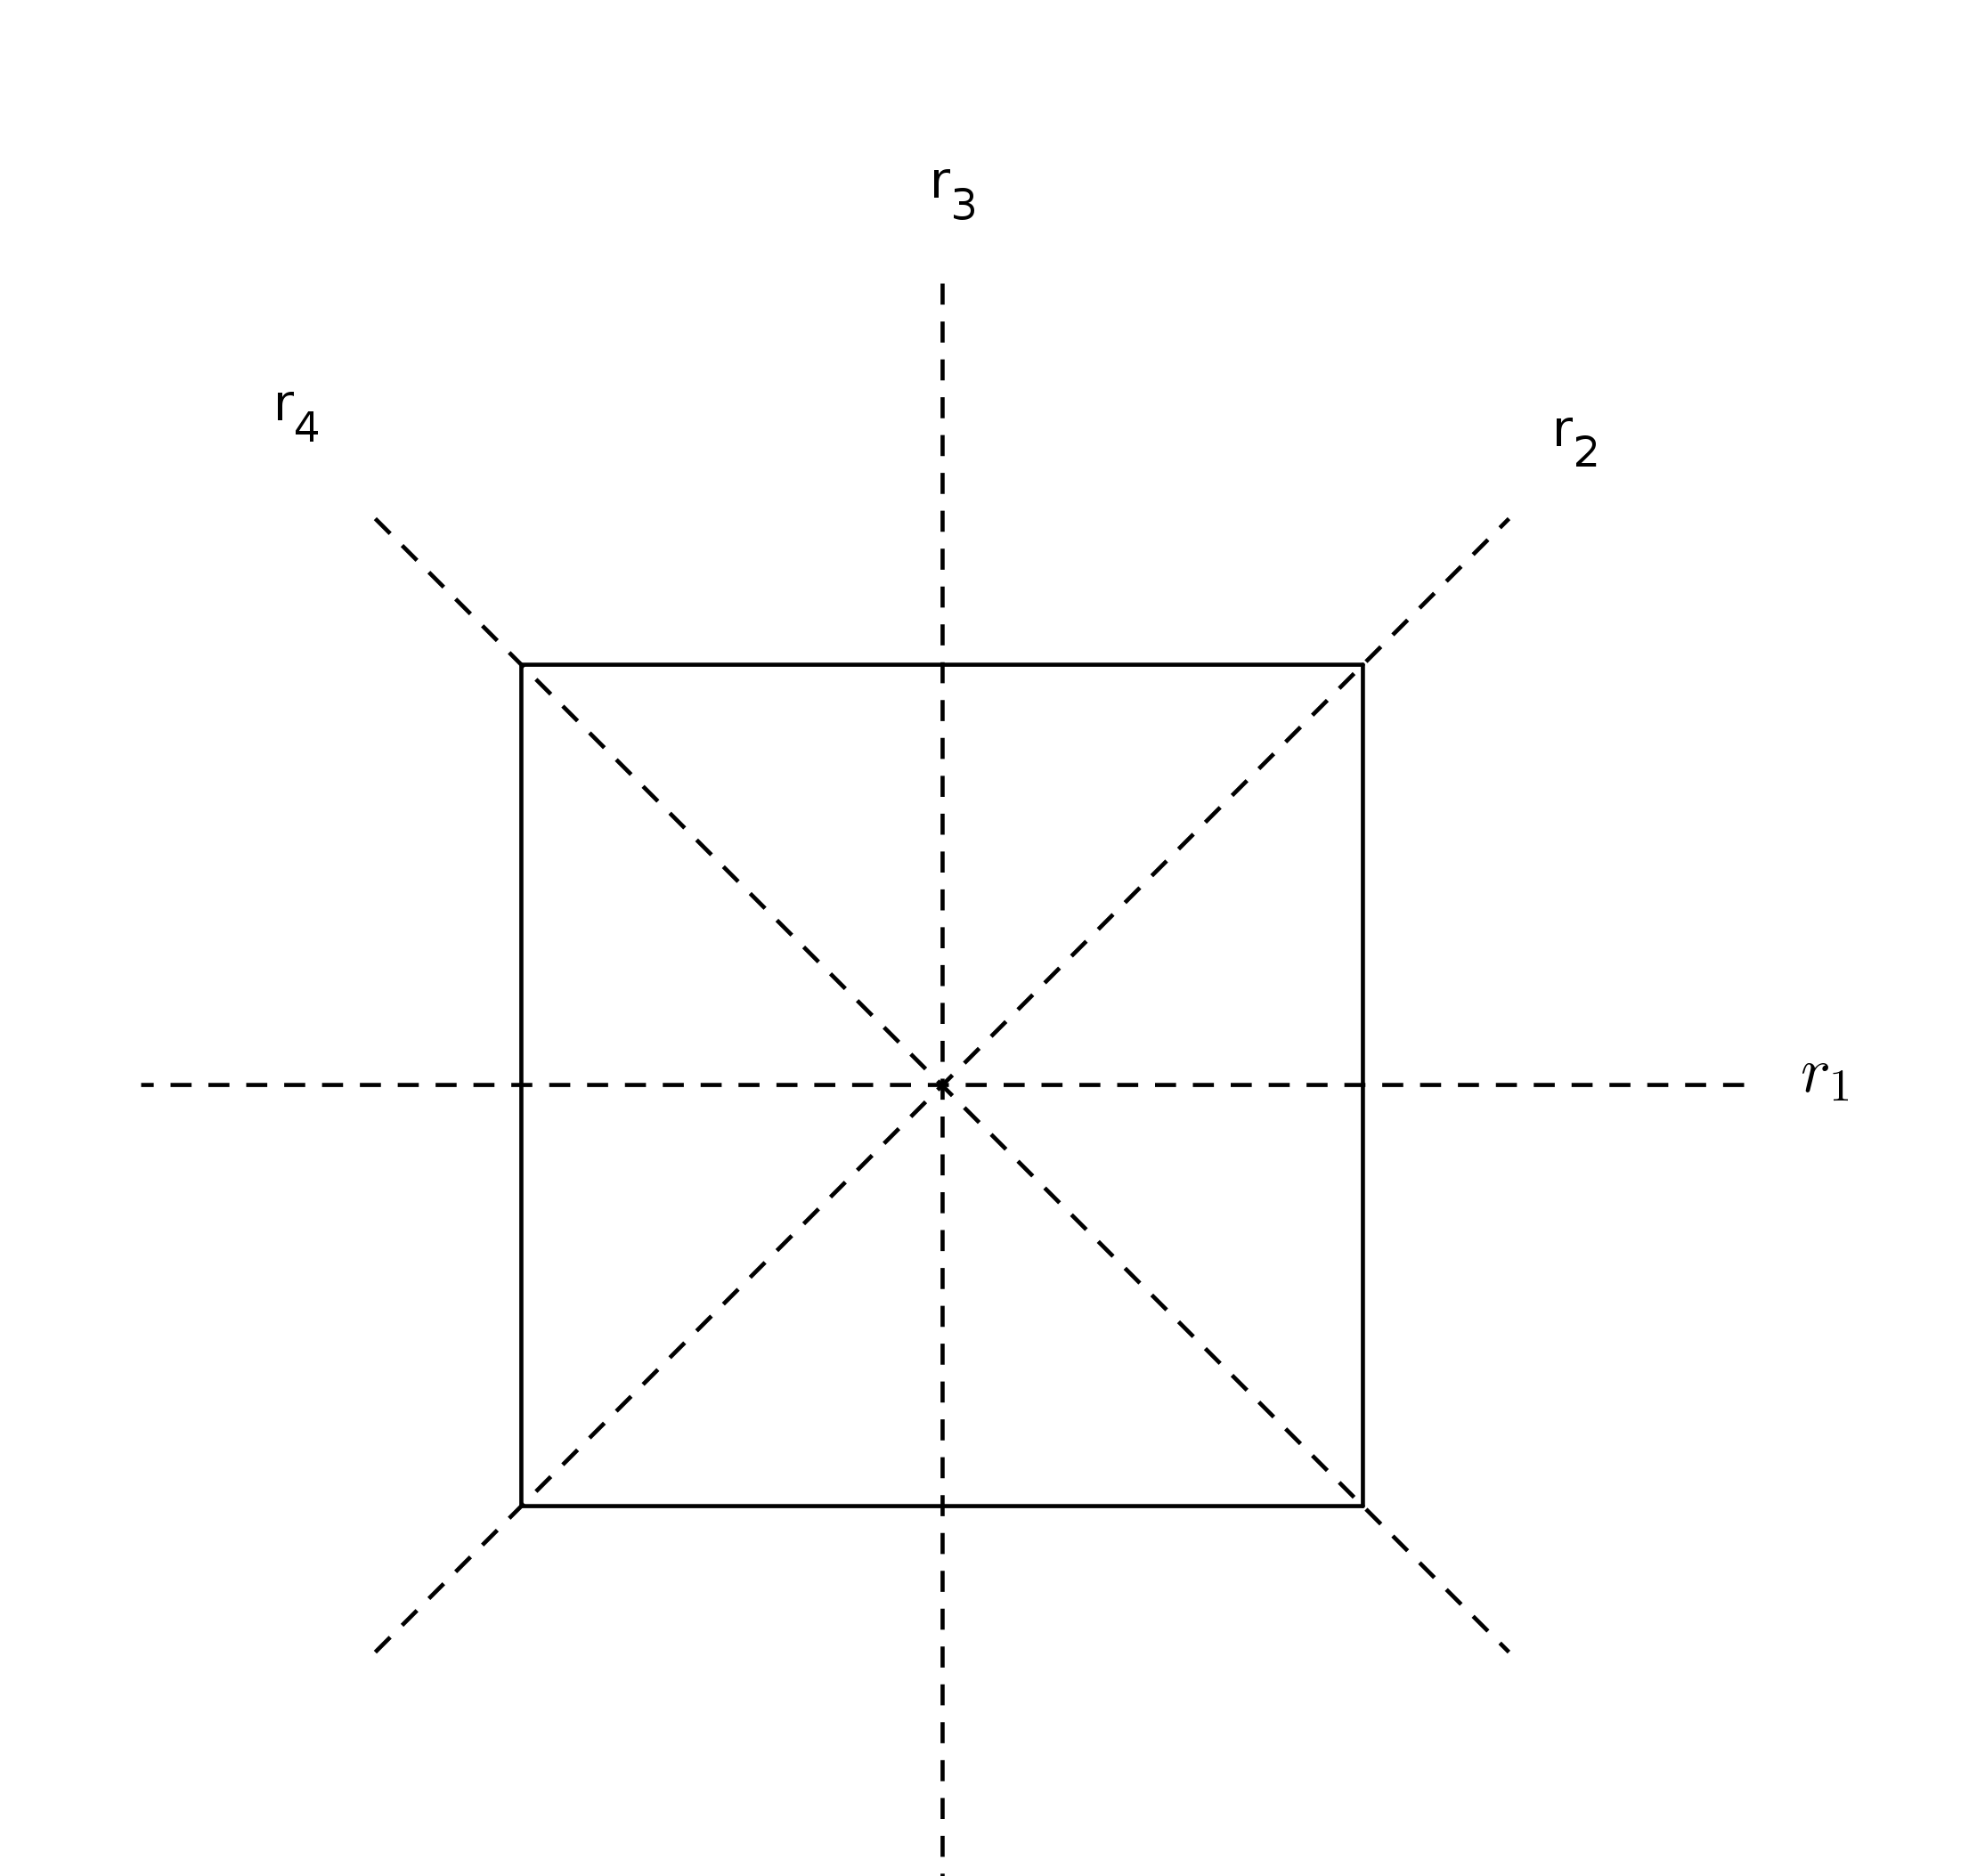
\includegraphics{cuadrado}
	  \captionsetup[figure]{textfont = normal, labelformat=empty, labelsep=period}
	  \vskip 1.80em
  	  \caption*{Fuente: elaboración propia con programa para computadora geogebra.}
  \label{fig:ejemplo}
\end{figure}
Sea $a$ la rotación de ángulo $\frac{\pi}{2}$ y $b$ la reflexión a través del eje $r_2$. Es fácil ver, bajo consideraciones geométricas, que cualquier otro elemento de este grupo se puede obtener por medio de $a$ y $b$.

De manera mas abstracta, este grupo, que es llamado grupo diédrico de orden ocho y usualmente denotado por $D_4$, puede ser definido con dos generadores que satisfacen las relaciones
\begin{equation*}
a^4 = 1, \quad b^2 = 1 , \quad baba = 1.  
\end{equation*}
Por lo tanto este grupo puede ser descrito  como 
\begin{equation*}
D_4 = \{ 1, a, a^2, a^3, b, ab, a^2b, a^3b \}. 
\end{equation*}
Como todas los elementos de este grupo están en terminos de $a$ y $b$, entonces para encontrar una representación matricial $A \colon D_4 \to GL(n,K)$ sobre el campo $K$, será suficiente encontrar matrices $A(a)$, $B(b)$ tales que $A(a)^4 = I$, $A(b)^2 = I$, $A(b)A(a)A(b)A(a) = I.$

Es fácil determinar representaciones de grado uno para $D_4$ en un campo $K$ de característica diferente a dos, de la siguiente manera:
\begin{equation*}
\begin{aligned}
A(a) & = 1\\
B(a) & = 1 \\ 
C(a) & = -1 \\
D(a) & = -1
\end{aligned}
\qquad 
\begin{aligned}
A(b) & = 1\\
B(b) & =  -1 \\
C(b) & = 1 \\
D(b) & = -1.
\end{aligned}
\end{equation*}
Pensando en el significado geométrico de $a$ y $b$, como dos funciones del plano al plano, se puede calcular sus matrices con respecto a la base canónica para obtener otra representación matricial de $D_4$:
\begin{equation*}
\begin{aligned}
W(a) = \begin{pmatrix}
0 & -1 \\
1 & 0
\end{pmatrix}
\end{aligned}
\qquad \text{,} \qquad
\begin{aligned}
W(b) &= \begin{pmatrix}
 0 & 1 \\
 1 & 0
\end{pmatrix}. 
\end{aligned}
\end{equation*}
\end{ejemplo}

\begin{ejemplo}[Suma directa de representaciones]
Sean $T \colon G \to GL(V)$ y $S \colon G \to GL(W)$ dos representaciones de un grupo $G$ sobre un anillo conmutativo $R$. Se puede definir una nueva representación $V \oplus W$, que es llamada la \textbf{suma directa} de dos representaciones dadas y se denota como $T \oplus S$, de la siguiente manera: \begin{equation*} (T \oplus S)_g = T_g \oplus S_g, \quad \mbox{para cada } g \in G. \end{equation*}

Si se eligen bases $\{v_1, \dots, v_n\}$ y $\{ w_1, \dots, w_m \}$ de $V$ y $W$ respectivamente y se denota por $g \mapsto A(g)$ y $g \mapsto B(g)$ las correspondientes representaciones matriciales en las bases dadas, entonces la representación matricial asociada a $T \oplus S$ con respecto a la base $\{ (v_1,0), \dots , (v_n), (0,w_1), \dots, (0,w_n)  \}$ de $V \oplus W$, viene dada por
\begin{equation*} g \mapsto \begin{pmatrix}
A(g) & 0 \\
0 & B(g)
\end{pmatrix}. \end{equation*}
\end{ejemplo}
Los ejemplos anteriormente expuestos sirven de motivación para introducir algunos conceptos de teoría de la representación. En este trabajo se restringirán las representaciones al caso en el cual $R$ es un campo, debido a que con este caso se logra ilustrar la relación de teoría de representación con los problemas de grupo-anillos.

Primero considérese $T \colon G \to GL(V)$ una representación de un grupo $G$ sobre un campo $K$ y asúmase que $\phi \colon V \to W$ es un isomorfismo de espacios vectoriales sobre $K$. Entonces se puede definir una nueva representación $\overline{T} \colon G \to GL(W)$ por medio de $\overline{T_g} \colon \phi \circ T_g \circ \phi^{-1}$ para todo $g \in G$. Esto es, esencialmente, una copia de $T$. La relación entre estas dos representaciones está ilustrada en el diagrama de la figura \ref{fig:ejemploSumaRepresentaciones}, 
\begin{figure}[t]
  \centering
  \caption{\hskip 2em \textbf{Diagrama conmutativo para representaciones equivalentes}}
  	  \vskip -0.59em 
  	  \[\xymatrix { V \ar[r]^{T_g} 
  	  \ar[d]_{\phi}
  	   & V \ar[d]^{\phi} \\
  	  W \ar[r]_{\overline{T_g}} & W}\]
	  \captionsetup[figure]{textfont = normal, labelformat=empty, labelsep=period}
	  \vskip 0.20em
  	  \caption*{Fuente: elaboración propia con programa para computadora \textbf{xymatrix}.}
  \label{fig:ejemploSumaRepresentaciones}
\end{figure}
lo cual sugiere la siguiente:
\begin{definicion}
Dos representaciones $T \colon G \to GL(V)$ y $\overline{T} \colon G \to GL(W)$ de un grupo $G$ sobre el mismo campo $K$ se dicen que son \textbf{equivalentes} si existe un isomorfismo $\phi \colon V \to W$ tal que $\overline{T_g} = \phi T_g \phi^{-1} $ para cualquier $g \in G$.
\end{definicion}
\begin{definicion}
Dos representaciones matriciales $A \colon G \to GL(n,K)$ y $B \colon G \to GL(n,K)$ de un grupo $G$ sobre un campo $K$ se dicen \textbf{equivalentes} si existe una matriz invertible $U \in GL(n,K)$ tal que $A(g) = UB(g)U^{-1}$ para cualquier $g \in G$.
\end{definicion}

\begin{ejemplo}\label{ejemciclico}
Sea $G$ un grupo cíclico de orden $m$ y $K$ un campo que contiene a $\{ \xi_1, \xi_2, \dots, \xi_m \}$, el conjunto de todas las raíces distintas de la unidad de orden $m$. Entonces, si se consideran las representaciones $B$ y $\Gamma$ dadas en el ejemplo \ref{rciclica} con 
\begin{equation*} \mathsf{U} = \begin{pmatrix}
\xi_1 & \xi_1^2 & \cdots & \xi_1^m \\
\xi_2 & \xi_2^2 & \cdots & \xi_2^m \\
 & & \cdots & \\
 \xi_m & \xi_m^2 & \cdots & \xi_m^m \\ 
\end{pmatrix}. \end{equation*}
Es claro que $\mathsf{U} \in GL(n,K)$, ya que $\mathsf{U}$ es una matriz de Vandermonde con $det(\mathsf{U}) = \prod_{1 \leq i < j \leq m}(\xi_i - \xi_j) \neq 0$. Entonces, calculando, por un lado se tiene 
\begin{equation*} B(a)\mathsf{U} = \begin{pmatrix}
\xi_1 & 0 & \cdots & 0\\
0 & \xi_2 & \cdots & 0\\
 & & \cdots & \\
 0 & 0 & \cdots & \xi_m
\end{pmatrix} \begin{pmatrix}
\xi_1 & \xi_1^2 & \cdots & \xi_1^m \\
\xi_2 & \xi_2^2 & \cdots & \xi_2^m \\
 & & \cdots & \\
 \xi_m & \xi_m^2 & \cdots & \xi_m^m
\end{pmatrix} = \begin{pmatrix}
\xi_1^2 & \xi_1^3 & \cdots & \xi_1 \\
\xi_2^2 & \xi_2^3 & \cdots & \xi_2 \\
 & & \cdots & \\
\xi_m^2 & \xi_m^2 & \cdots & \xi_m
\end{pmatrix}, \end{equation*} similarmente \begin{equation*} 
\mathsf{U}\Gamma(a) = 
\begin{pmatrix}
\xi_1 & \xi_1^2 & \cdots & \xi_1^m \\
\xi_2 & \xi_2^2 & \cdots & \xi_2^m \\
 & & \cdots & \\
 \xi_m & \xi_m^2 & \cdots & \xi_m^m \\
\end{pmatrix}
\begin{pmatrix}
0 & 0 & \cdots & 1 \\
1 & 0 & \cdots & 0 \\
 & & \cdots & \\
0 & 0 & \cdots & 1 \\
\end{pmatrix} = \begin{pmatrix}
\xi_1^2 & \xi_1^3 & \cdots & \xi_1 \\
\xi_2^2 & \xi_2^3 & \cdots & \xi_2 \\
 & & \cdots & \\
\xi_m^2 & \xi_m^2 & \cdots & \xi_m
\end{pmatrix}
\end{equation*} con lo que se ha demostrado que $A(g) = \mathsf{U}B(g)\mathsf{U^{-1}}$, para cualquier $g \in G$ y concluye que $B$ y $\Gamma$ son equivalentes. 
\end{ejemplo}

Considérese $T \colon G \to GL(V)$ una representación de un grupo $G$ sobre el campo $K$, con espacio de representación $V$ y supóngase que $V$ contiene un subespacio $W$ que es invariable bajo $T$, esto es, un subespacio tal que $T_g(W) \subset W$, para cualquier $g \in G$. Entonces se puede considerar el homomorfismo de grupos que asigna a cada elemento $g \in G$ la restricción de $T_g$ al subespacio $W$. Por ser $T_g$ la restricción, es claro que el homomorfismo anterior es una representación de $G$ sobre $K$, con espacio de representación $W$.

Con el afán de dar una representación matricial de este hecho, considérese una base $\{ w_1, w_2, \dots, w_t \}$ de $W$ y extiéndase a una base $ \{ w_1, \cdots, w_t, v_{t+1}, \cdots, v_n \}$ de $V$. Entonces la matriz asociada a cada función $T_g$, $g \in G$ con respecto a esa base es de la forma
\begin{equation*} \begin{pmatrix}
A(g) & B(g) \\
0 & C(g)
\end{pmatrix} \end{equation*} donde $A(g) \in GL(t,K), C(g) \in GL(n-t,K)$ y $B(g)$ es una matriz de $t \times (n-t)$. Estas consideraciones sugieren la siguiente:
\begin{definicion}
Una representación $T \colon G \to GL(V)$ de un grupo $G$ sobre un campo $K$ es llamada \textbf{irreducible} si los únicos subespacios propios de $V$ que son invariantes bajo $T$ son los triviales, es decir, $V$ y $\{ 0 \}$.
\end{definicion}

La representación es llamada \textbf{reducible} si $V$ contiene  subespacios no triviales que son invariantes bajo $T$. 

\begin{definicion}
Una representación matricial $M \colon G \to GL(n,K)$ es llamada \textbf{reducible} si existe una matriz $\mathsf{U} \in GL(n,K)$ tal que para cualquier $g \in G$, se tiene que la matriz $\mathsf{U}M(g)U^{-1}$ es de la forma
\begin{equation*}
\mathsf{U}M(g)U^{-1} = \begin{pmatrix}
A(g) & B(g) \\
0 & C(g)
\end{pmatrix}. 
\end{equation*}  
\end{definicion}

El ejemplo \ref{ejemciclico} muestra que la representación regular de un grupo cíclico de orden $m$, sobre un campo $K$ que contiene raíces de la unidad de orden $m$ es reducible. De hecho, cualquier representación regular de un grupo finito $G \neq \{ 1 \}$ sobre cualquier campo es reducible. En efecto, nótese que si en el espacio de representación $RG$ se toma el elemento $\hat{G} = \sum_{g \in G}g$ entonces $ T_g(\hat{G}) = \hat{G}$ por lo tanto el subespacio generado por $\hat{G}$ es invariante bajo $T$ y $(\hat{G}) \neq RG.$  

\begin{definicion}
Una representación $T \colon G \to GL(V)$ de un grupo $G$ sobre un campo $K$ es llamada \textbf{completamente reducible} si para todo subespacio $W$ que es invariante bajo $T$ existe un subespacio invariante $W'$ tal que $V = W \oplus W'$.
\end{definicion}
Para entender de mejor manera esta definición se dará una interpretación en términos de matrices.

Sea $\{ w_1, w_2, \dots, w_t \}$ y $\{ w_{t+1}, \dots, w_n\}$ bases dadas para $W$ y $W'$ respectivamente, entonces $\{ w_1, w_t, w_{t+1}, \dots, w_n \}$ es una base de $V$ y para cualquier $g \in G$ la matriz de $T_g$ con respecto a esta base es de la forma
\begin{equation*} \begin{pmatrix}
A(g) & 0 \\
0 & B(g)
\end{pmatrix} \end{equation*} donde $A(g)$ y $B(g)$ son las matrices de representación de $T_g$ en $W$ y $W'$ con respecto a las bases dadas. 

\begin{definicion}
Una representación matricial $M \colon G \to GL(n,K)$ es llamada completamente reducible si cualquier representación matricial $M$ de la forma 
\begin{equation*} \begin{pmatrix}
A(g) & B(g) \\
0 & C(g)
\end{pmatrix} \end{equation*} es equivalente a una representación matricial de la forma
\begin{equation*} \begin{pmatrix}
A(g) & 0 \\
0 & D(g) 
\end{pmatrix}. \end{equation*}
\end{definicion}


\section{\hskip 1em Representación y Módulos.}
 En este sección se estudiará la conexión que hay entre módulos y representaciones. Dicha conexión se establece usando el concepto de grupo-anillo.
 
 \begin{proposicion}\label{prop:biyeccionModulos}
 Sea $G$ un grupo y $R$ un anillo conmutativo con unidad. Entonces, existe una biyección entre representaciones de $G$ sobre $R$ y $RG\mbox{-módulos}$ libres y de rango finito. 
 \end{proposicion}
 \begin{proof*}
 Dada una representación $T \colon G \to GL(V)$ de $G$ sobre $R$, se asocia a ella el $RG\mbox{-módulo}$ construido a partir de $V$ manteniendo la misma estructura aditiva y definiendo el producto de un elemento $v \in V$ por un escalar $\alpha = \srg{g}{G}{a} \in RG$ como 
 \begin{equation}\label{defproducto}
 \alpha v = \left( \srg{g}{G}{a}  \right)v = \sum_{g \in G}a(g)T_g(v).
 \end{equation}
 
 Usando está definición de producto se verifica:
 \begin{bulletList}
 \newItem Distributividad de la suma de escalares respecto al producto por escalar \begin{eqnarray*}
  (\alpha + \beta)v &=& \left( \sum_{g \in G}(a_g + b_g)g  \right)v \\
   &=& \sum_{g \in G}(a_g + b_g)T_g(v) \\
   &=& \sum_{g \in G}a_gT_g(v) + \sum_{g \in G}b_gT_g(v) \\
    &=& \alpha v + \beta v .
 \end{eqnarray*}
 \newItem Distributividad de la  suma de elementos del módulo respecto al producto por escalar
 \begin{eqnarray*}
 \alpha(v + w) &=& \left(\srg{g}{G}{a}(v + w)  \right) \\
  &=& \sum_{g \in G}a_gT_g(v+w) \\
  &=& \sum_{g \in G}a_gT_g(v) + \sum_{g \in G}a_gT_g(w) \\
  &=& \alpha v + \alpha w .
 \end{eqnarray*}
 \newItem Para la asociatividad, por un lado se tiene
 \begin{eqnarray*}
 \alpha(\beta v) &=& \left( \sum_{h \in G}a(g)h \right)\left( \sum_{g \in G}b(g)T_g(v) \right) \\
  &=& \sum_{h \in G}a(h)T_h\left( \sum_{g \in G}b(g)T_g(v)  \right) \\
  &=& \sum_{h, g \in G}a(h)b(g)T_{hg}(v).
 \end{eqnarray*}
 
 Por otro lado se tiene
 \begin{eqnarray*}
 (\alpha\beta)v &=& \left( \sum_{h,g \in G}a(h)b(g)hg  \right)(v)\\
  &=& \sum_{h,g \in G}a(h)b(g)T_{hg}(v)
 \end{eqnarray*}
 con lo que se comprueba que $\alpha(\beta v) = (\alpha\beta)v$.
 \newItem Considérese $\alpha = 1_{G}$, entonces
 \begin{eqnarray*}
 \alpha v &=& T_{1_G}(v)\\
  &=& I(v) \\
  &=& v.
 \end{eqnarray*}
 \end{bulletList}
  Por lo expuesto anteriormente es fácil notar que la multiplicación por escalar definida en la ecuación~\eqref{defproducto} induce un $RG\mbox{-módulo}$.
 
 Al converso, si $M$ es un $RG\mbox{-módulo}$ de rango finito sobre $R$, se define la representación de $G$ sobre $R$ asignando a cada elemento $g \in G$ el $R\mbox{-automorfismo}$ $T_g \colon M \to M$ dado por $T_g(m) = gm$.
 
 Nótese que dado $T \colon G \to GL(V)$ una representación de $G$ sobre $R$ y $M$ su $RG\mbox{-módulo}$ inducido, se tiene que $S$, la representación inducida por $M$, es tal que $S_g(m) = gm = \alpha m \simeq T_g(m)$, donde $\alpha$ es la imagen de la inmersión de $G$ en $RG$ dada en el teorema \ref{inmersion}.
 
 De manera similar, dado $M$ un $RG\mbox{-módulo}$ y $S \colon G \to GL(M)$ su representación inducida, entonces su $RG\mbox{-módulo}$ inducido por la ecuación~\eqref{defproducto} deja invariante a $M$. Por lo tanto se ha demostrado que las aplicaciones construidas anteriormente son inversas la una de la otra. 
 \end{proof*}
  Como ejemplo considérese  un grupo finito $G$ y $RG$ como un módulo sobre sí mismo, de esta forma $RG$ es de rango finito $|G|$ sobre $R$. Entonces, dado un elemento $x \in G$, la representación $T_x \colon RG \to RG$ viene dada por: \begin{equation*}T_{x}\left( \sum_{g \in G}a(g)g\right) = x\left( \sum_{g \in G}a(g)g\right) = \left( \sum_{g \in G}a(g)gxg\right).\end{equation*}
  
  Esto significa que $x \in G$ actúa en los elementos de la base $G = \{ g_1, \dots, g_n \}$ multiplicándolos por la izquierda. En otras palabras, la representación asociada al $RG\mbox{-módulo}$ $RG$ es precisamente la representación regular de $G$. 
\begin{lema}
  Sea $T \colon G \to GL(V)$ una representación de un grupo $G$ sobre un campo $K$, con espacio de representación $V$, entonces un subespacio $W \subset V$ es invariante bajo $T$ si y sólo si $W$ es un $KG\mbox{-módulo}$ de $V$. 
  \end{lema}
  \begin{proof*}
  Se procede a demostrar este hecho en dos partes:
  \begin{bulletList}
  \newItem Sea $W \subset V$ invariante bajo $T$, entonces $T_{g}(W) = W$ para cualquier $g \in G$. Sean $w_1, w_2 \in W$ se tiene que $T_{g}(w_1 + w_2) = T_{g}(w_1) + T_{g}(w_2) \in W$, así $T_{g}^{-1}(T_{g}(w_1 + w_2)) \in W$. Por otra parte, si se considera $\alpha = \sum_{g \in G}a(g)g$ entonces $\alpha w = \sum_{g \in G}a(g)T_g(w) \in W$ y por lo tanto $W$ es un $KG\mbox{-módulo}$ de~$V$.
  \newItem Sea $W$ subespacio de $V$, $W \subset V$ y $W$ un $KG\mbox{-módulo}$ de $V$, entonces para $w \in W$ y $g \in RG$ se tiene $gw = 1\cdot T_g(w) \in W$. \qedhere
  \end{bulletList} 
  \end{proof*}
  
  \begin{teorema}\label{teo:relacionTG}
  Sea $G$ un grupo y $K$ un campo. Entonces:
  \begin{bulletList}
  \newItem Dos representaciones $T$ y $T'$ de $G$ sobre $R$ son equivalentes si y sólo si los correspondientes $RG\mbox{-módulos}$ son isomorfos.
  \newItem Una representación es irreducible (o completamente reducible) si y sólo si el correspondiente $RG\mbox{-módulo}$ es irreducible (o completamente reducible).
  \end{bulletList}
  \end{teorema}
  \begin{proof*}
  Se procede a demostrar este lema por incisos:
  \begin{bulletList}
  \newItem Supóngase que $T$ y $T'$ son representaciones de $G$ sobre $K$ equivalentes, entonces existe $\phi \colon V \to W$ isomorfismo, donde $V$ y $W$ son los espacios de representación de $T$ y $T'$ respectivamente, tal que $T'_g = \phi T_g \phi^{-1}$ para cualquier $g \in G$. Entonces se probará que $\phi$ es isomorfismo de $RG\mbox{-módulos}$ también.  En efecto
  \begin{eqnarray*}
   \phi(\alpha v) &=& \phi\left( \sum_{g \in G}a(g)T_g(v) \right) \\ 
   &=&  \sum_{g \in G}a(g)\phi(T_g(v)) \\
    & =& \sum_{g \in G}a(g)T'_g(\phi(v))\\ 
    &=& \alpha \phi(v).
  \end{eqnarray*}
   \newItem Supóngase que $M$ y $N$ son $RG\mbox{-módulos}$ isomorfos, entonces existe $f \colon M \to N$ isomorfismo de $RG\mbox{-módulos}$. Sean $T$ y $T'$ las representaciones inducidas por $M$ y $N$ respectivamente, entonces:
   \begin{eqnarray*}
   (fT_gf^{-1})(n) &=& 
    f\left(T_g\left(f^{-1}(n)\right)\right)\\
    &=& f\left(gf^{-1}(n)\right) \\
    &=& gf\left(f^{-1}(n)\right) \\
    &=& gn \\
    &=& T'_g(n)
   \end{eqnarray*} con lo que se comprueba que $T$ y $T'$ son equivalentes. 
   
   \newItem Si una representación $T$ es irreducible, entonces los únicos subespacios de $V$ que son invariantes bajo $T$ son los triviales y, por el lema anterior, los únicos submódulos de $M$, el módulo inducido por $T$, son los los triviales. De manera análoga se puede demostrar el converso. \qedhere
   \end{bulletList}
  \end{proof*}
  También es posible notar que si un $RG\mbox{-módulo}$ $M$ admite una descomposición como suma directa de submódulos $M = \oplus_{i = 1}^{t}M_i$ y si $T$ y $T_i$ denota las representaciones correspondientes a estos módulos, entonces $T = \oplus_{i = 1}^tT_i$. 
 
 En lo que sigue, se mostrará como la información que ya se conoce acerca de los grupo-anillos se puede trasladar a términos de representaciones de grupos. 
 
 El lector deberá recordar que en el corolario \ref{cor:car}, como consecuencia directa del teorema de Maschke, se demostró que si $K$ es un campo tal que $\car(K) \nmid |G|$, entonces $KG$ es un anillo semisimple. Además, se demostró en el teorema \ref{teo:wa} que en este caso todo $KG\mbox{-módulo}$ es simple. Por lo tanto, en particular, se sigue inmediatamente que todo $KG\mbox{-módulo}$ finito dimensional sobre $K$ se puede escribir como suma directa de módulos irreducibles.
 
 En términos de representaciones, esto significa que bajo estas condiciones, toda representación de $G$ sobre $K$ es la suma directa de representaciones irreducibles. Así, para determinar todas las representaciones de $G$ sobre $K$, mediante equivalencia, es suficiente determinar todos los $KG\mbox{-módulos}$ irreducibles, salvo isomorfismos. 
 
 Ahora, es necesario hacer uso del teorema de Wedderburn-Artin aplicado a grupo-anillos (teorema \ref{teo:wa}), el cual establece que el número de $KG\mbox{-módulos}$ irreducibles que no son isomorfos entre sí, es precisamente el número de componentes simples de $KG$ y estas están determinadas exclusivamente por la estructura de $KG$. En particular, es importante recordar que si se escribe $KG$ en la forma
 \begin{equation*} KG \simeq \oplus_{i = 1}^{r}M_{n_i}(D_i) \end{equation*} donde $D_i, 1\leq i \leq r$, son anillos de división que contienen a $K$ en sus centros, y si se calcula la dimensión en ambos lados de la ecuación, se tiene
 \begin{equation*} |G| = \sum_{i = 1}^{r}n_{i}^2[D_i:K]. \end{equation*}
 
 Por otro lado, se sabe que el módulo irreducible $I_i$ correspondiente a la componente simple $M_{n_i}(D_i)$ es isomorfo a $D_{i}^{n_i}$. Como el grado de la correspondiente representación $T_i$ viene dado por la dimensión de este módulo sobre $K$, se obtiene que
 \begin{equation*}  \grado (T_i) = [D_{i}^{n_i}:K] = n_i[D_i:K] \end{equation*} así, se puede escribir \begin{equation*} |G| = \sum_{i = 1}^{r}n_i\grado(T_i). \end{equation*} 
 
 \begin{ejemplo}
 Se mostró  en el ejemplo \ref{ejem:orden7} que si $G = \langle a \rangle$ denota al grupo cíclico de orden siete, entonces
 \begin{equation*} \mathds{Q}G \simeq \mathds{Q}\oplus\mathds{Q}(\zeta), \end{equation*} donde $\zeta$ denota una raíz primitiva de la unidad de orden siete. De lo anterior, las componentes simples de $\mathds{Q}G$ son anillos de matrices de $1\times 1$ sobre los anillos $\mathds{Q}$ y $\mathds{Q}(\zeta)$ respectivamente y por ende existen solamente dos representaciones irreducibles que no son equivalentes, $S$ y $T$ de $G$ sobre $\mathds{Q}$, con grados
 \begin{equation*} \grado(S) = [\mathds{Q}:\mathds{Q}] = 1, \quad \grado(T) = [\mathds{Q}:\mathds{Q}] = 6. \end{equation*} 
 
 Como las representaciones $1\mbox{-dimensionales}$ son equivalentes si y sólo si son iguales y como cualquier grupo admite la representación trivial $S \colon G \to GL(1,\mathds{Q})$ dada por $S_g = 1$, para cada $g \in G$, entonces la representación $1\mbox{-dimensional}$ de $G$ sobre $\mathds{Q}$ es la trivial.
 
 Para determinar $T_a$, de acuerdo a las consideraciones anteriores, se debe considerar el $\mathds{Q}G\mbox{-módulo}$ irreducible $I_2 = D_2^{n_2}$ correspondiente a la segunda componente simple de $\mathds{Q}$. Entonces, la representación $T \colon G \to GL(I_2)$ está dada por $T_a(v) = av$, para cada $v \in I_2$. En este caso, $n_2 = 1$ y $D_2 = \mathds{Q}(\zeta)$, así que $I_2 = \mathds{Q}(\zeta)$, donde la multiplicación por un elemento $\alpha = (\alpha_1, \alpha_2) \in \mathds{Q}G$ está dada por $\alpha v = \alpha_2v$, para todo $v \in \mathds{Q}(\zeta)$. Recordando que el elemento $a \in \mathds{Q}(\zeta)$ le corresponde, vía isomorfismo, el elemento $(1,\zeta) \in \mathds{Q}\oplus\mathds{Q}(\zeta)$ se tiene
 \begin{equation*} T_a(v) = av = \zeta v, \quad v 
 \in \mathds{Q}(\zeta). \end{equation*} Por lo tanto, si se toma $\{ 1, \zeta, \zeta^2, \dots, \zeta^5 \}$ como una base de $\mathds{Q}(\zeta)$ sobre $\mathds{Q}$, entonces la correspondiente matriz está dada por
 \begin{equation*} A(a) = \begin{pmatrix}
 0 & 0 & 0 & 0 & 0 & -1 \\
 1 & 0 & 0 & 0 & 0 & -1 \\
 0 & 1 & 0 & 0 & 0 & -1 \\
 0 & 0 & 1 & 0 & 0 & -1 \\
 0 & 0 & 0 & 1 & 0 & -1 \\
 0 & 0 & 0 & 0 & 1 & -1
 \end{pmatrix}. \end{equation*}
 \end{ejemplo}
 \begin{ejemplo}[Representaciones del grupo diédrico de orden ocho.]
 Se ha probado en ele ejemplo \ref{ejem:diedrico} que el grupo $D_4$ admite cuatro representaciones distintas de grado uno y una representación $W$ de grado dos sobre $\mathds{Q}$, por lo tanto existen cuatro componentes simples isomorfas a $\mathds{Q}$. Sean $M_n(D)$ la componente simple correspondiente a la representación de grado dos. Como $2 = \grado(W) = n[D:\mathds{Q}]$, entonces $n = 1$ y $[D:\mathds{Q}]$ o $n = 2$ y $[D:\mathds{Q}] = 1$.
 
 Para el primer caso, se puede observar que $\mathds{Q}D_4$ debe ser de la forma \begin{equation*} \mathds{Q}D_4 \simeq \mathds{Q} \oplus \mathds{Q} \oplus \mathds{Q}\oplus\mathds{Q}\oplus D\oplus D',\end{equation*} donde $D'$ es una anillo de división con $[D':\mathds{Q}] = 2$. Es fácil notar que un anillo de división de dimensión dos sobre un campo tiene que ser conmutativo, entonces $\mathds{Q}D_4$ es conmutativo, lo cual es una contradicción, ya que $D_4$ no es abeliano. 
 
 En consecuencia, se debe tener que $n = 2$ y $D = \mathds{Q}$. De esta forma \begin{equation*}  \mathds{Q}D_4 \simeq \mathds{Q}\oplus\mathds{Q}\oplus\mathds{Q}\oplus\mathds{Q}\oplus M_{2}(\mathds{Q}). \end{equation*}
 \end{ejemplo}
 

